\section{Projektbeschreibung}

Cloud Provider bieten verschiedenste virtuelle Instanzen auf physischen Hosts
an. Dabei nutzt jeder virtuelle Server die vorhandenen Ressourcen des
physischen Systems unterschiedlich. Hier kommt es, aufgrund der
Mischkalkulation für die Ressourcen, zu einer Überbuchung (Overcommitment) des
Hosts. Weil das Monitoring nicht ausreichend ist, oder kein sinnvolles
Placement implementiert ist (Placement beschreibt den Algorithmus der einen
Node ermittelt auf dem eine neue virtuelle Instanz angelegt wird) kommt es
regelmäßig zu Performanceeinbußen. Für Kunden gibt es keine Transparenz über
die ihm zugeteilten und durch ihn genutzten Ressourcen, weshalb auch keine
ressourcenbasierte Abrechnung erfolgen kann. Teamleiter sind häufig mit der
Effizienzsteigerung der Plattform beschäftigt und müssen die Auslastung
steigern. Dies ist ohne detaillierte Auslastungsreports nicht möglich.

In diesem Projekt soll eine funktionierende Open Source Software entwickelt
werden, die sich in drei Teile gliedert:
\begin{outline}
  \1 Die verschiedenen Ressourcetypen (CPU Zeit / Daten Durchsatz / RAM
  Auslastung / Speicher Auslastung / Netzwerk Durchsatz) der einzelnen
  virtuellen Server müssen in einem sinnvollen Intervall periodisch ermittelt
  werden.
  \1 Die Daten müssen aggregiert und gespeichert werden. Hierbei ist auf eine
  Skalierung auf mindestens 10.000 virtuelle Instanzen unter Berücksichtigung
  der Verfügbarkeit und Performance der Datenbank zu achten (Sharding oder
  Replikation, verteilt oder zentral, dokumentenbasiert oder relational).
  \1 Diese Daten können dann dem Endanwender präsentiert werden (API und
  Web-UI). Hierzu wird eine Userstory Erhebung unter den drei Anwendertypen
  Kunde, Administrator, Manager bei Partnerunternehmen durchgeführt, um
  gewünschte Algorithmen zur Visualisierung zu ermitteln (z.b. ermitteln von
  freien oder überbuchten Nodes, grafische Auswertung für Kunden).
  \1 Die anfallenden Daten müssen aggregiert werden. Für Marketing- und
  Analysezwecke sind Daten über eine Zeitspanne von einem Jahr hilfreich, diese
  müssen aber nicht granular sein. Für andere Anwendungsfälle (z.B.
  Fehleranalyse) werden granulare Daten über die letzten zwei bis vier Wochen
  benötigt. Das optimale Aggregationsverhalten muss im Verlauf des Projekts
  ermittelt werden.
\end{outline}

\section{Output}

Der Kunde bekommt einen besseren Überblick über sein monatliches / tägliches
Nutzungsverhalten und kann seine genutzten Produkte besser verwalten. Der
Serveradministrator kann einen besseren Betrieb ermöglichen, indem er mit Hilfe
der Daten z.B. entscheidet:
\begin{outline}
    \1 ob ein Hostsystem überlastet ist und ggf. virtuelle Maschinen auf andere
       Server umziehen müssen. Steigert die verfügbare Leistung pro Instanz und
       somit die Kundenzufriedenheit, ohne dass das Unternehmen in mehr Hardware
       investieren muss.
    \1 welches Hostsystem am besten für einen Neukunden geeignet ist.
    \1 ob eine Neuanschaffung von Hardware sinnvoll ist.
    \1 ob die eingebaute Hardware ggf. einen Hardwarerefresh benötigt.
\end{outline}

Das Marketing, bzw. der Vertrieb, kann die Daten nutzen um z.B.:
\begin{outline}
    \1 gezieltere Kampagnen für Server-Upgrades, bzw. den Verkauf von teureren
       Serverpaketen (mehr RAM / Kerne / Speicher) durchzuführen
    \1 inaktiven Kunden aufgrund der Historie ein besseres Angebot zu
       unterbreiten.
    \1 neue Produkte nach “Pay-what-you-Use” Prinzip anzubieten. Dies könnte dem
       Unternehmen einen Marktvorsprung gegenüber anderen Unternehmen in der
       Branche bieten.
\end{outline}

\section{Mögliche negative Nebeneffekte}

Je nach Anzahl der verwendeten Hostsysteme in einem Netzwerk könnte die interne
Netzwerkübertragung überlastet werden. Aufgrund dessen muss geprüft werden,
welcher Übertragungsintervall der Nutzungsdaten von den einzelnen Hostsystemen
an die Datenbank sinnvoll ist. Außerdem muss hier evaluiert werden, ob Daten
zur zentralen Instanz geschickt werden oder diese die Daten selbst abholen
soll.

\section{Qualitätsmanagement}
Für das Qualitätsmanagement werden die Techniken und Werkzeuge des Continuous
Integration (CI) und Continuous Delivery (CD) zum Einsatz kommen. Continuous
Integration unterstützt dabei den Entwickler der Software durch einen von ihm
vordefinierten Testkatalog, welcher bei jeder Softwareänderung in einer
Testmatrix ausgeführt wird. Dieser Vorgang gibt dem Entwickler ein direktes
Feedback über die Funktionstüchtigkeit der Software, so ist er nicht auf ein
manuelles Testverfahren angewiesen. Sobald die Tests erfolgreich abgeschlossen
worden sind, kann die vollständig funktionierende Software mit Hilfe von
Continuous Delivery auf verschiedenen Test- oder Produktivumgebungen
bereitgestellt werden. Ein Akzeptanztest der Benutzeroberfläche durch eine
Anwender-Testgruppe markiert das Erreichen eines Meilensteins und schließt
somit eine Projektphase der Projektplanung ab. Durch dieses Vorgehen wird nur
am Ende jeder Projektphase ein manuelles Eingreifen in den Testablauf benötigt.

\section{Qualitätsanforderungen}
\centering
\raisebox{-5cm}{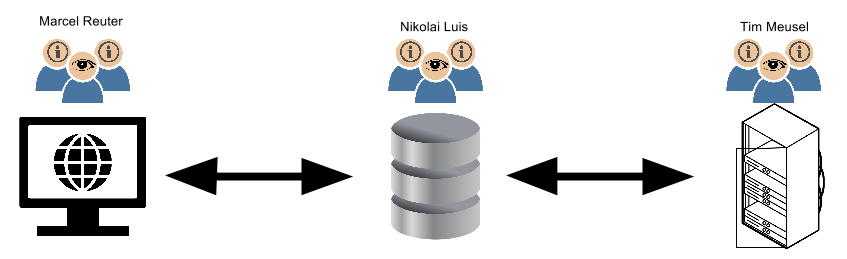
\includegraphics[width=\textwidth]{roles.png}}
\\[1.5cm]
\small
\makebox[\textwidth]{%
    \begin{tabular}{lp{.33\textwidth}p{.33\textwidth}p{.33\textwidth}}
      \toprule
      & WebFrontend & Datenhaltung & Datenbeschaffung \\
      \midrule
      Muss
      &
        Ausgewählten Benutzern Informationen über die Nutzung von einzelnen VMs oder
        Hosts in Form von Grafiken und Statistiken anzeigen.
                    &
                      Eine dauerhafte Bereitstellung und Verarbeitung von mehreren tausend Datensätzen
                      garantieren
                                   &
                                     Die verschiedenen Ressourcentypen eines einzelnen virtuellen Servers in einem
                                     sinnvollen Zeitrahmen periodisch ermitteln. \\
      Soll
      &
        Den Systemadministrator bei Neukonfigurationen unterstützen.
                    &
                      Eine einfache Input- und Output-Schnittstelle verfügen,
                      über die Datensätze ein- und ausgelesen werden können.
                                   &
                                     Die ermittelten Daten in möglichst kürzester
                                     Zeit an die Datenhaltung liefern. \\
      Kann
      &
        Bereitstellen einer Schnittstelle zum ausführen komplexer Abfragen und Analysen
        -- nach Bedarf mit Visualisierung
                    &
                      Die Daten auf einer bereits aggregierten Ebene Drittsystemen über eine API
                      anbieten. Die Daten nach aktuellen Sicherheitstandards (Verschlüsselungen)
                      übertragen.
                                   &
                                     Die Daten bei möglichen Ausfällen der gesamten Datenhaltung,
                                     kurzfristig selber speichern und anschließend der gesamten
                                     Datenhaltung nachliefern. \\

      \bottomrule
    \end{tabular}
}


%%% Local Variables:
%%% mode: latex
%%% TeX-master: "prd-de"
%%% End:
